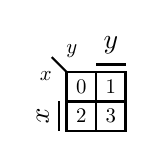
\begin{tikzpicture}[scale=0.75]
\def\sc{0.75};
\draw[thick] (0,0) -- ++(1,0) -- ++(0,1) -- ++(-1,0) -- cycle;
\draw[thick] (0,0.5) -- ++(1,0);
\draw[thick] (0.5,0) -- ++(0,1);
\draw[thick] (0,1) -- (-0.25,1.25);
\draw (-0.125,1.125) node[anchor=north east,scale=0.75]{$x$};
\draw (-0.125,1.125) node[anchor=south west,scale=0.75]{$y$};
\draw[thick] (-0.125,0) to node[sloped,below,rotate=180]{$x$} (-0.125,0.5);
\draw[thick] (0.5,1.125) to node[sloped,above]{$y$} (1,1.125);
\draw (0.25,0.25) node[scale=\sc]{2};
\draw (0.25,0.75) node[scale=\sc]{0};
\draw (0.75,0.25) node[scale=\sc]{3};
\draw (0.75,0.75) node[scale=\sc]{1};
\end{tikzpicture}